\section{Comportement}
\begin{frame}
  \begin{columns}[T]
    \begin{column}{.5\textwidth}
      \begin{itemize}
        \item Implémentation d'une machine d'état
        \item Trois états :
          \begin{itemize}
            \item Endormi
            \item Recherche de visage
            \item Suivi de visage
          \end{itemize}
        \item Manque de temps pour plus développer
      \end{itemize}
    \end{column}
    \begin{column}{.5\textwidth}
      \begin{figure}
        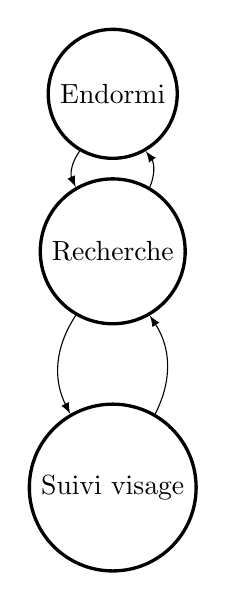
\begin{tikzpicture}[scale = 0.5]
 \tikzset{directed/.style={<-}} 
  \node[draw,circle, very thick] (Sleep) at (0,8) {Endormi};
  \node[draw,circle, very thick] (FaceSearch) at (0,4) {Recherche};
  \node[draw,circle, very thick] (FaceFollow) at (0,-2) {Suivi visage};
  \draw[->,>=latex] (Sleep) to[bend right] (FaceSearch);
  \draw[->,>=latex] (FaceSearch) to[bend right] (FaceFollow);
  \draw[->,>=latex] (FaceSearch) to[bend right] (Sleep);
  \draw[->,>=latex] (FaceFollow) to[bend right] (FaceSearch);





\end{tikzpicture}

      \end{figure}
    \end{column}
 \end{columns}
\end{frame}

